% Geometry, font
\documentclass[12pt, letter]{article}
\usepackage[margin=0.8in]{geometry}
\usepackage[T1]{fontenc}
\usepackage{fourier}
\usepackage{titling}
\setlength{\droptitle}{-5em} 
\usepackage[parfill]{parskip}
\usepackage{graphicx}
\graphicspath{{imgs/}}
\usepackage{hyperref}

\usepackage{fancyhdr}
\lhead{ECE 4542: Advanced Engineering Algorithms}
\rhead{Zach Neveu}
\pagestyle{fancy}

% Math stuff
\usepackage{amssymb}
\usepackage{bm}

% Code Highlighting
\usepackage{minted}
\usemintedstyle{solarizedlight}

\title{ Homework 5 }

\begin{document}
\maketitle
\thispagestyle{fancy}

\begin{enumerate}
	\item 5-6 Statements about pure IP and LP relaxation
	\begin{enumerate}
		\item False. The feasible region for an IP problem is a subset of points within the feasible region for the LP relaxation, not the other way around. In other words $F_{IP} \in F_{LP}$
		\item True. If the LP solution is integral, then results for LP and ILP are identical.
		\item False. Assuming an arbitrary convex LP feasible region, a CPF is just as likely to round to a point outside of the IP feasible region as it is to round to a point inside the IP feasible region.
	\end{enumerate}
	\item 5-7 Assignment Problem
	\begin{enumerate}
		\item Use the assignees as branch points. For example, for the first node, create five branches corresponding to the 5 possible tasks the first person could be assigned to. To set an optimistic bound on results, take the remaining assignees and remaining tasks. For each task assign the cheapest assignee regardless of whether they end up performing multiple tasks. Once a feasible solution has been found, branches can be fathomed if their optimistic bound has higher cost than the already discovered solution. In order to quickly prune a large number of nodes, search the tree by assigning the cheapest available task to each task in a greedy fashion.
		\item Start by assigning person 1 to task 1 as this has the minimum cost. Bound is now 138. Assign person 2 to task 3 with cost 24. Bound is still 128. Assign person 3 to task 4 giving a bound of 146. Assign person 4 to task 2, giving a bound of 157. It turns out that person 5 can be assigned to task 5, hitting our bound of 157. Using this as the best found solution, it is possible to prune many branches. Working back through the list of decisions. Backtracking from person 5, to 4 to 3, it turns out that if person 3 is assigned to task 2, the bound is 154, which is less than 157 so should be explored. Exploring this path, it is possible to assign person 4 to task 4, and person 5 to task 5, achieving the exact bound of 154. Backtracking further up the decision tree, no further optimizations can be made, yielding the final assignments below and a total cost of 154.
	\end{enumerate}
	\begin{table}[h]
		\centering
		\caption{Final Assignments}
		\label{tab:label}
		\begin{tabular}{cc}
		Person & Task \\
		\hline
		1 & 1 \\
		2 & 3 \\
		3 & 2 \\
		4 & 4 \\
		5 & 5 \\
		\end{tabular}
	\end{table}
	\item 6-3a
	\begin{itemize}
		\item Start by branching to $x_1\le 1$ and $x_1\ge 2$
		\item Calculate respective LP Bounds of 7.5 (non-integral) and 14.22 (non-integral)
		\item Branch by $x_2 \le 1$ and $x_2 \le 2$ to give four regions
		\item $Z(x_1\le 1,x_2 \le 1) \le Z(1,1)=6$ (integral)
		\item $Z(x_1\ge 2, x_2 \le 1) = Z(2,1) = 11$ (integral)
		\item $Z(x_1 \le 1, x_2 \ge 2) = Z(1,2.5) = 7.5$ (non-integral)
		\item $Z(x_1 \ge 2, x_2 \ge 2) = Z(2.22,3.12) = 14.22$ (non-integral)
		\item Expand the highest region first into $x_1 \le 2$ and $x_1 \ge 3$
		\item First region has integral solution of 13, second region is infeasible.
		\item Solution of 13 allows other branches to all be pruned.
	\end{itemize}
	\begin{figure}[h]
		\centering
		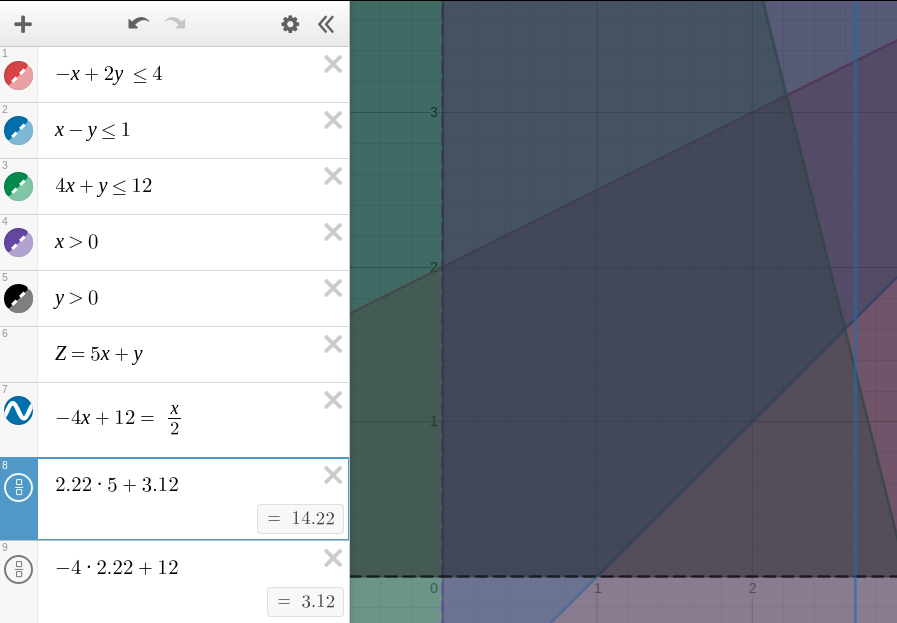
\includegraphics[width=0.8\textwidth]{6-8}
		\caption{Graphical Solution to 6-3a}
		\label{fig:6-8}
	\end{figure}

	\item 6-8
	\begin{itemize}
		\item Branch based on $x_1 \le 1$, $x_1 \ge 2$
		\item Branch based on $x_2 \le 1$, $x_2 \ge 2$
		\item Branch based on $x_3 \le 1$, $x_3 \ge 2$
		\item Branch based on $x_4 \le 1$, $x_4 \ge 2$
		\item Since objective increases positively with all variables, try branch where all largest first. This turns out to be infeasible.
		\item Work way downwards through values until optimal solution of $x_1=2, x_2=2, x_3=1, x_4=0$ found
	\end{itemize}
	\item 7-1a
	\begin{itemize}
		\item Fix $x_1=0$
		\item Fix $x_3=0$ 
	\end{itemize}
	\item 7-2a
	\begin{itemize}
		\item Fix $x_1=0$
	\end{itemize}
	\item 7-3
	\begin{itemize}
		\item Fix $x_3=0$ 
		\item First constraint redundant
		\item Fix $x_5=0$ 
		\item Fix $x_6=0$ 
		\item Third constraint redundant
	\end{itemize}
	\item 7-4
	\begin{enumerate}
		\item Redundant. $\sum x_i \le 5$
		\item Not redundant. If $x_1=1,x_2=0,x_3=1, \sum x_i > 5$
		\item Not redundant. $\sum x_i$ could be both $\le$ and $\ge$ 2
		\item Redundant. $\sum x_i$ is always $>-4$
	\end{enumerate}
\end{enumerate}

\end{document}
